Data goes through a particular path through the pipeline of a processor and typically, a pipeline is split up in multiple stages. With a lockstep processor, each of the stages are effectively working in parallel. Figure \ref{fig:pipelining} illustrates hardware pipelining for a \emph{Reduced Instruction Set Computer} (RISC) processor. The pipeline is split up in four or more stages, e.g. instruction fetch, instruction decode, execution and write-back stage. During the \emph{instruction fetch} (IF stage) an instruction is loaded from \emph{instruction memory} (IMEM), which is decoded in the \emph{instruction decode} (ID) stage where the type of operation is determined by the opcode and operands are identified by their register addressing, and finally, the operation is executed and the result is written back to the register file.

\begin{figure}[H]
\centering
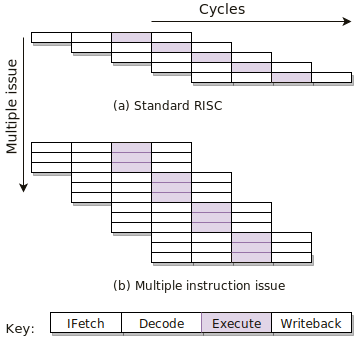
\includegraphics[width=.5\textwidth]{figures/pipelining}
\caption{Pipelining and multiple instruction issue\cite{tta_codegen}.}
\label{fig:pipelining}
\end{figure}

When bypassing is completely absent the result of an instruction can be obtained only after it is written back. On the other hand, with bypassing, a bypass network of wires and busses connects the execution and writeback stages back to the ID stage. We may forward a value using these wires or busses to the operands of an instruction. This way, we can obtain the result of an instruction before it has been written back to the register file. We illustrate this behaviour in Figure \ref{fig:bypass_problem}.

\begin{figure}[b!]
\centering
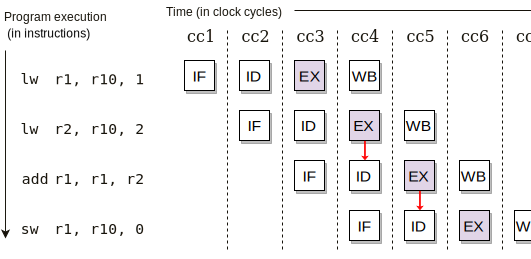
\includegraphics[width=.8\textwidth]{figures/bypassing_example}
\caption{Instructions being executed using the single-cycle data path, assuming pipelined execution.}
\label{fig:bypass_problem}
\end{figure}

Four consecutive instructions are executed of which the last two instructions have a RaW dependency with the instruction prior to it. As you can see in Figure \ref{fig:bypass_problem} the instructions prior to said instructions are in the execution stage when their result is required, namely, when said instruction are in the ID stage. We either need to stall for a cycle, such that the previous instruction is in the WB stage, or we need to forward the result from the execution stage to the ID stage. Since insertion of stall cycles results in less efficient code, we choose to forward the result using the bypass network (indicated with a vertical arrow from EX to ID).\\

%TODO: update picture, make nicer and have on top stages, and below remain almost the same
%\begin{figure}[H]
%\centering
%\subfloat{\includegraphics[width=.275\textwidth]{figures/bypass_prob_legend}}
%\hfil
%\subfloat{\includegraphics[width=.475\textwidth]{figures/bypass_problem}}
%\caption{Bypassing network differences between four stage and five stage pipeline configuration.}
%\label{fig:bypass_problem}
%\end{figure}
%TODO: replace with picture from presentation (03_nov)

With implicit bypassing (also called transparent bypassing), bypassing opportunities are detected and controlled by dedicated hardware on chip. However, doing this at run-time has some advantages and some disadvantages.
\begin{itemize}
\item \textbf{Advantage:} The compiler does not need to take data paths and the values that are in the pipeline into consideration, because bypassing is transparent to the compiler. This results in a less complex compiler.
%TODO: move up!!!!!
\item \textbf{Disadvantage:} 
If you push the responsibility of identifying and exploiting forwarding to the hardware, it needs $2\cdot d\cdot n$ comparators (where $d$ is the number of stages between ID en WB and $n$ the number of issue slots) to compare operands of an instruction to registers defined by previous instructions that are already in the pipeline. Altogether, this results in a more complex gate design and increased area.
\end{itemize}

It has been observed that values in a register file are often transient, meaning that they last only for a short time.  









